% !TEX root = ./article.tex

\documentclass{article}

\usepackage{mystyle}
\usepackage{myvars}



%-----------------------------

\begin{document}

	\maketitle % Insert title

	\thispagestyle{fancy} % All pages have headers and footers


%-----------------------------
%	ABSTRACT
%-----------------------------

	\begin{abstract}
		\noindent [TODO ]
	\end{abstract}

%-----------------------------
%	TEXT
%-----------------------------


	\section{Introducción}
	\label{sec:introducción}

		\subsection{Máquinas de Vectores Soporte}
		\label{sec:support-vector-machine}

			\paragraph{}
			[TODO ]

	\section{Experimento sobre conjunto de datos sencillo}
	\label{sec:e1}

		\paragraph{}
		[TODO ]

		\begin{table}[H]
			\centering
			\begin{tabu}{ | c | c | c |}
				\hline
				\multicolumn{3}{ | c | }{Simple Dataset} \\ \hline
				\bfseries $x_1$ & \bfseries $x_2$ & \bfseries $d(x)$
				\csvreader[head to column names]{../datasets/simple.csv}{
					1=\one, 2=\two, 3=\three
				}
				{\\\hline\one&\two&\three}
				\\\hline
			\end{tabu}
			\caption{Conjunto de datos Simple}
			\label{table:e1_dataset}
		\end{table}

		\begin{figure}[h]
			\begin{center}
				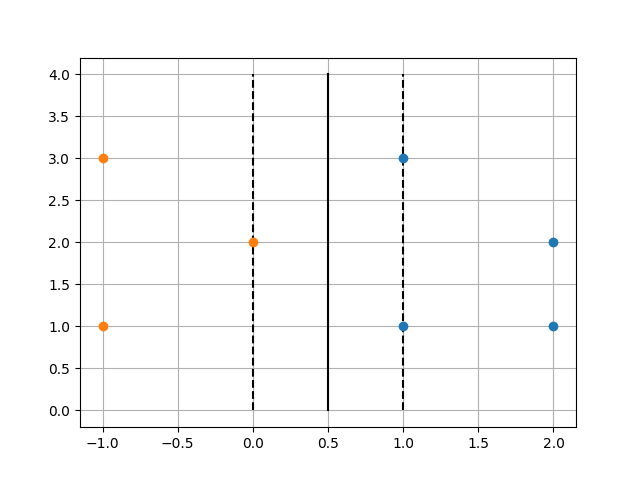
\includegraphics[width=0.75\textwidth]{graph}
			\end{center}
			\caption{[TODO ]}
			\label{fig:e1_plot}
		\end{figure}


	\section{Experimento sobre Wine Dataset}
	\label{sec:e2}

		\paragraph{}
		[TODO ]
		\csvreader[
		  longtable=| c | c |,
		  table head=\hline\bfseries \# Grado &\bfseries Tasa de Error \\\hline,
			table foot= \caption{[TODO]}\label{table:so-e1}\\,
		  late after line=\\\hline,
		  before reading={\catcode`\#=12},after reading={\catcode`\#=6}
		]{../results/results.csv}{1=\k,2=\error}{\k & \error}

		\paragraph{}
		[TODO ]

		\begin{figure}
			\begin{center}
				\begin{tikzpicture}
					\begin{axis}[
						% only scale the axis, not the axis including the ticks and labels
						scale only axis=true,
						% set `width' and `height' to the desired values
						width=0.9\textwidth,
						height=0.3\textwidth,
						]
						\addplot table [x=k, y=error, col sep=comma] {../results/results.csv};
					\end{axis}
				\end{tikzpicture}
			\end{center}
			\caption{[TODO ]}
			\label{plot:sol-e1}
		\end{figure}

		\paragraph{}
		[TODO ]

		\begin{table}
			\centering
			\small
			\begin{tabu}{ | c | c | }
				\hline
				\multicolumn{2}{ | c | }{SVM con kernel gausiano} \\ \hline
				Datos & Tasa de Error \\ \hline
				Pruebae								& $0.016393$	\\
				\hline
			\end{tabu}
			\caption{[TODO ]}
			\label{table:e3}
		\end{table}
%-----------------------------
%	Bibliographic references
%-----------------------------
	\nocite{subject:taa}
	\nocite{garciparedes:machine-learning-support-vector-machine}
	\nocite{dataset:wine}
  \bibliographystyle{alpha}
  \bibliography{bib/bib}

\end{document}
